\documentclass[11pt, a4paper]{article}

\usepackage{graphicx}
\usepackage[a4paper,top=3cm,bottom=2cm,left=2cm,right=2cm,marginparwidth=1.75cm]{geometry}
\usepackage[english]{babel}
\usepackage[utf8x]{inputenc}
\usepackage{subfig}
\usepackage{amsmath}
\usepackage{amssymb}

\graphicspath{ {./images} }
\newcommand*{\qed}{\hfill\ensuremath{\quad\square}}%
\newcommand*{\rad}{\ensuremath{\,\text{rad}}}
\newcommand*{\R}{\ensuremath{\mathbb{R}}}

\makeatletter
\renewcommand*\env@matrix[1][*\c@MaxMatrixCols c]{%
  \hskip -\arraycolsep
  \let\@ifnextchar\new@ifnextchar
  \array{#1}}
\makeatother

\newtheorem{theorem}{Theorem}

%------------------------------------------------
%Templates for images and figures
% \begin{figure}[h]
%   \centering
%   \subfloat[caption 1]{{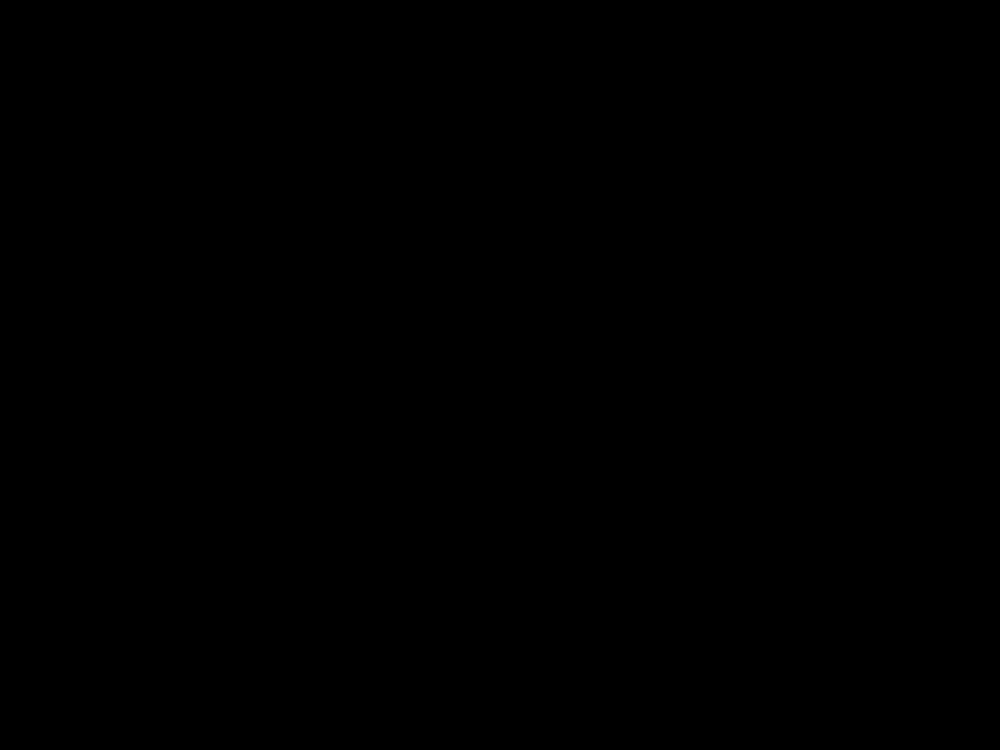
\includegraphics[width=30mm]{images/placeholder.png}}}%
%   \qquad
%   \subfloat[caption 2]{{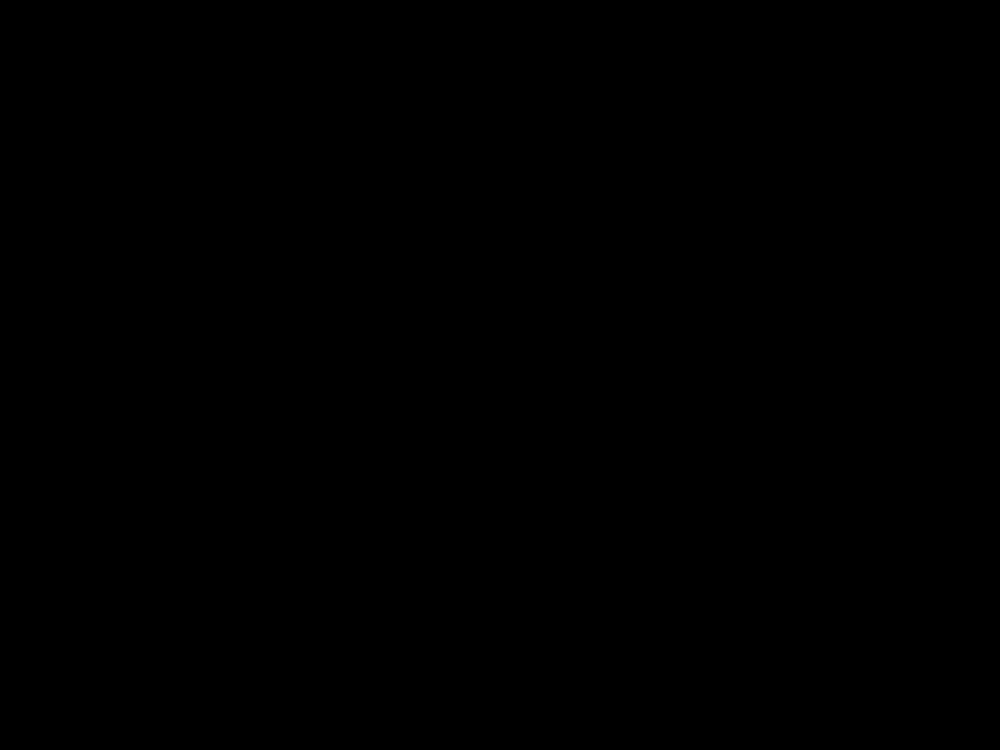
\includegraphics[width=30mm]{images/placeholder.png}}}%
%   \caption{Description}
% \end{figure}

% \begin{figure}[h]
%   \centerline{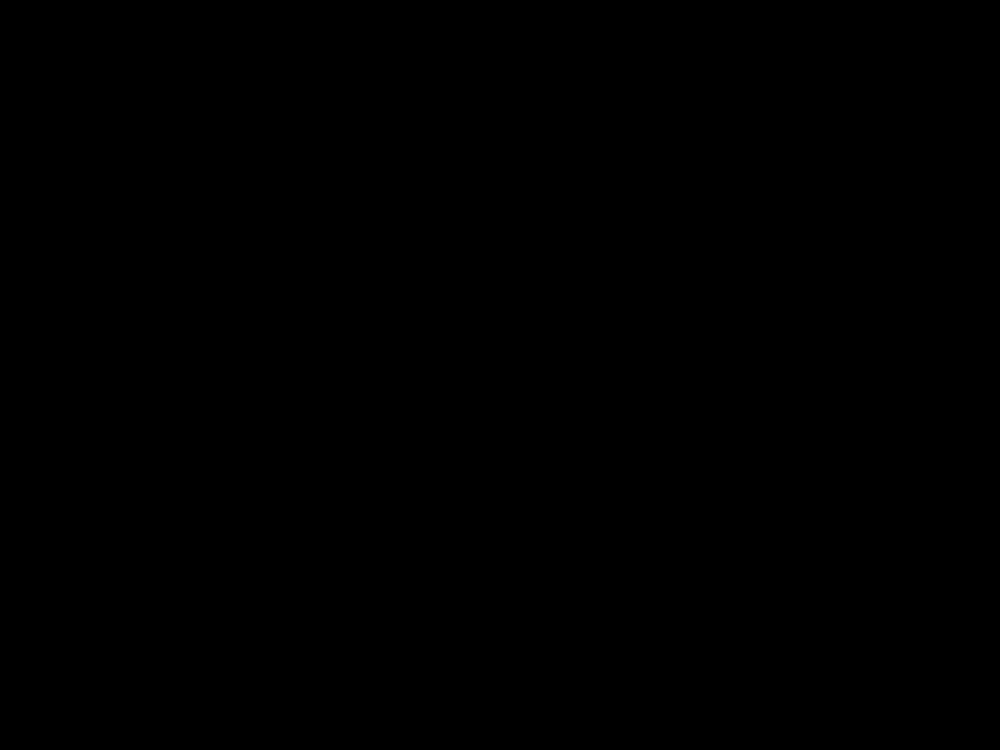
\includegraphics[width=50mm]{images/placeholder.png}}
%   \caption{Description}
% \end{figure}
%-----------------------------------------------

\begin{document}
\setcounter{section}{1}
\setcounter{equation}{0}

\section{Thermofluids Lecture 2: First law of thermodynamics (23/04/2020)}


\subsection{The first law for a closed system}
The first law of thermodynamics for a closed system takes the following form:
\begin{equation}
  \Delta KE + \Delta PE + \Delta U = Q - W
\end{equation}
Where $\Delta KE$ is the kinetic energy, $\Delta PE$ is the potential energy, $\Delta U$ the internal energy, $Q$ heat and $W$ the work done.


\subsection{Internal energies of a system}
The internal energies of a system are a microscopic phenomena. Examples of this are kinetic energy of atoms (translational and rotational), vibrations of atoms, chemical energies, nuclear energy, lattice energy, etc. Though statisical mechanics has gone a long way in explaining the exact nature of these internal energy we usually do not concern ourselfs with these in classical thermodynamics. Instead we make a simplified approximation of the total sum of these energies, which is close enough for the systems we concern ourselfs with in classical thermodynamics. The equation for internal energy used in classical thermodynamics is:
\begin{equation}
  U = cmT
\end{equation}
where $c$ is the heat capacity.


\subsection{Heat and work in thermodynamics}
Mechanical work done is usually described with the following integral:
\begin{equation}
  W = \int_{s1}^{s2} \vec{F}\cdot d\vec{s}
\end{equation}
However note that the work done as described by the integral is dependent on the path taken. In other words, it is a process variable. Because of the scope of classical thermodynamics only concerning itself with systems in equilibrium in time indendent states usually use the following integral notation:
\begin{equation}
  W = \int_1^2 \delta W
\end{equation}
Where the $\delta$ is used to denote an inexact differential. Using this $\delta$ automatically implies path dependence which in the scope of classical thermodynamics cannot be expressed. Note the expression for the first law where the LHS contains only state variables, while the RHS only contains process variables.


\subsection{A thermodynamic cylinder system}
SIDE NOTE: THIS SECTION NEEDS TO BE IMPROVED LATER
Consider a cylinder with a volume $V$. The gas inside this cylinder has a pressure $p$. The work done by the plunger moving back a distance of $x$ can be described with the following equations:
\begin{gather}
  F = pA\\
  \delta W_{12} = F\,ds = pA\,dx = p\,dV
\end{gather}
\begin{gather}
  \delta W = p\,dV, \quad dU = mc\,dT\\
  -p\,dV = dU\\
  -\delta W = dU
\end{gather}
\begin{figure}[h!]
  \centerline{\includegraphics[width=50mm]{images/Work Done.png}}
  \caption{Situation of the moving plunger}
\end{figure}
\end{document}